\begin{center}
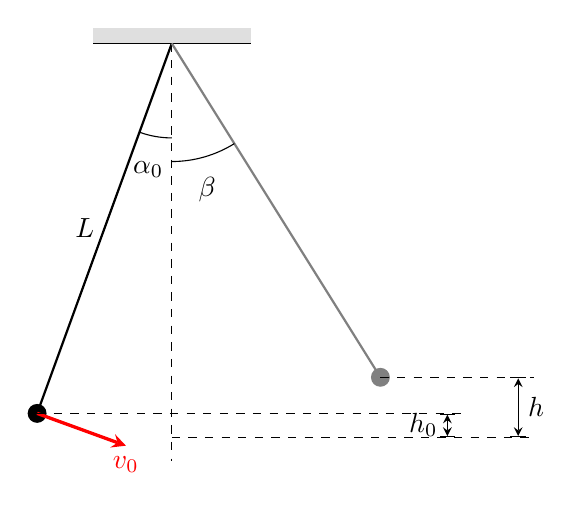
\begin{tikzpicture}[>=stealth]
 \fill[gray!25] (-1,0) rectangle (1,0.2);
 \draw (-1,0) -- (1,0);
 \draw[dashed] (0,0) -- (0,-5.3);
 \draw[thick] (0,0) -- (-110:5) node[midway, left] {$L$};
 \draw[thick, gray] (0,0) -- (-58:5);
 \fill (-110:5) circle (0.12);
 \fill[gray] (-58:5) circle (0.12);
 \draw[->, very thick, red] (-110:5) -- ++(-20:1.2) node[below] {$v_0$};
 \draw (0,-1.2) arc (-90:-110:1.2);
 \node at (-0.3,-1.6) {$\alpha_0$};
 \draw (0,-1.5) arc (-90:-58:1.5);
 \node at (0.45,-1.85) {$\beta$};
 \draw[dashed] (0,-5) -- (4.6,-5);
 \draw[dashed] (-1.71,-4.70) -- (3.7,-4.70);
 \draw[dashed] (2.65,-4.24) -- (4.6,-4.24);
 \draw[|<->|] (3.5,-5) -- (3.5,-4.70) node[midway, left] {$h_0$};
 \draw[|<->|] (4.4,-5) -- (4.4,-4.24) node[midway, right] {$h$};
\end{tikzpicture}
\end{center}
(Winkel übertrieben gezeichnet.) Wir messen die Höhen vom tiefsten Punkt der Bahn aus. Beim Start liegt die Pendelmasse um
\begin{align}
 h_0 &= \hnpF = \Lp\cdot\left(1-\cos\alpO\right) = \hnp
\end{align}
über dem tiefsten Punkt. Im Umkehrpunkt auf der anderen Seite ist die Geschwindigkeit null; die Energieerhaltung $m\,g\,h_0 + \frac{1}{2}m\,v_0^2 = m\,g\,h$ ergibt
\begin{align}
 h &= \hpF \\
   &= \Lp\cdot\left(1-\cos\alpO\right)+\frac{\left(\vnp\right)^2}{2\cdot\gE} \\
   &= \hp \approx \result{\hpP{-2}{2}}
\end{align}
über dem tiefsten Punkt. Das entspricht einer Auslenkung von
\begin{align}
 \beta &= \bepF = \bep \approx \result{\bepP{0}{2}}
\end{align}
